\section{A Web Application for Optimization and Visualization}
\label{sec:web-app}
In order to make this optimization framework available to researchers, students, and anyone who would prefer not to work with the code itself, I developed a web application that implements its major components.
I developed this tool using the python library ``Streamlit" \citep{streamlit}, which facilitates the transformation of algorithms and visualizations to a web application.
Fortunately for the developer, coding in Streamlit web framework requires no handling of html, javascript, or other distractions.
Instead, Streamlit provides tools for converting Python code directly into interactive tables and plots.

This web application is initialize with a choice of three models and four data-sets (Figure \ref{fig:web-app-1}), although it would be straight-forward to add additional ones.

\begin{figure}
\begin{center}
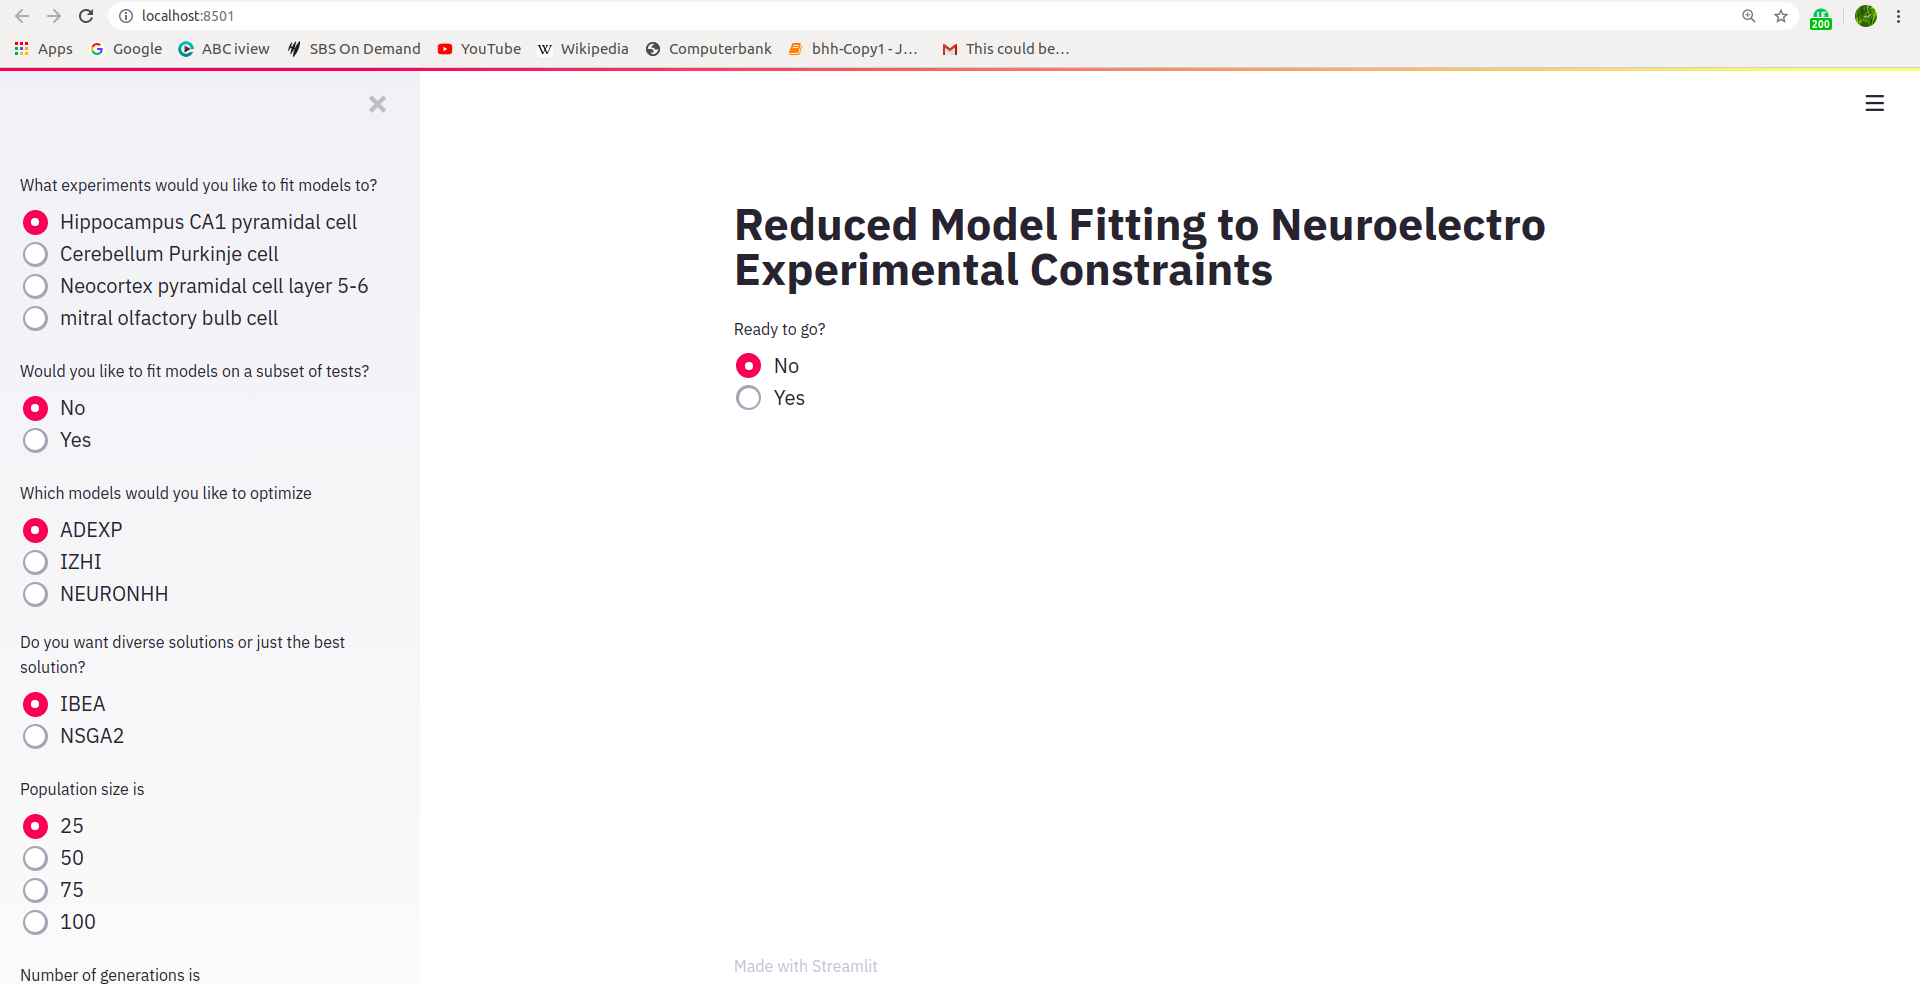
\includegraphics[scale=1]{chapters/app_tex/web_app_thesis}
\end{center}
\caption[Web Application (1)]{\textbf{A Web Application for Optimization: Part A}.
I created a web application to guide a user through the entire optimization process for reduced neuron models.
The side-pane of the web application provides users with a choice of three models, and four data sets that can be used to fit data.
}
\label{fig:web-app-1}
\end{figure}

The user is given a choice of very simple optimisation choices including what model type to use and the experimental data that will be used to guide the optimizer (Figure \ref{fig:web-app-2}).

\begin{figure}
\begin{center}
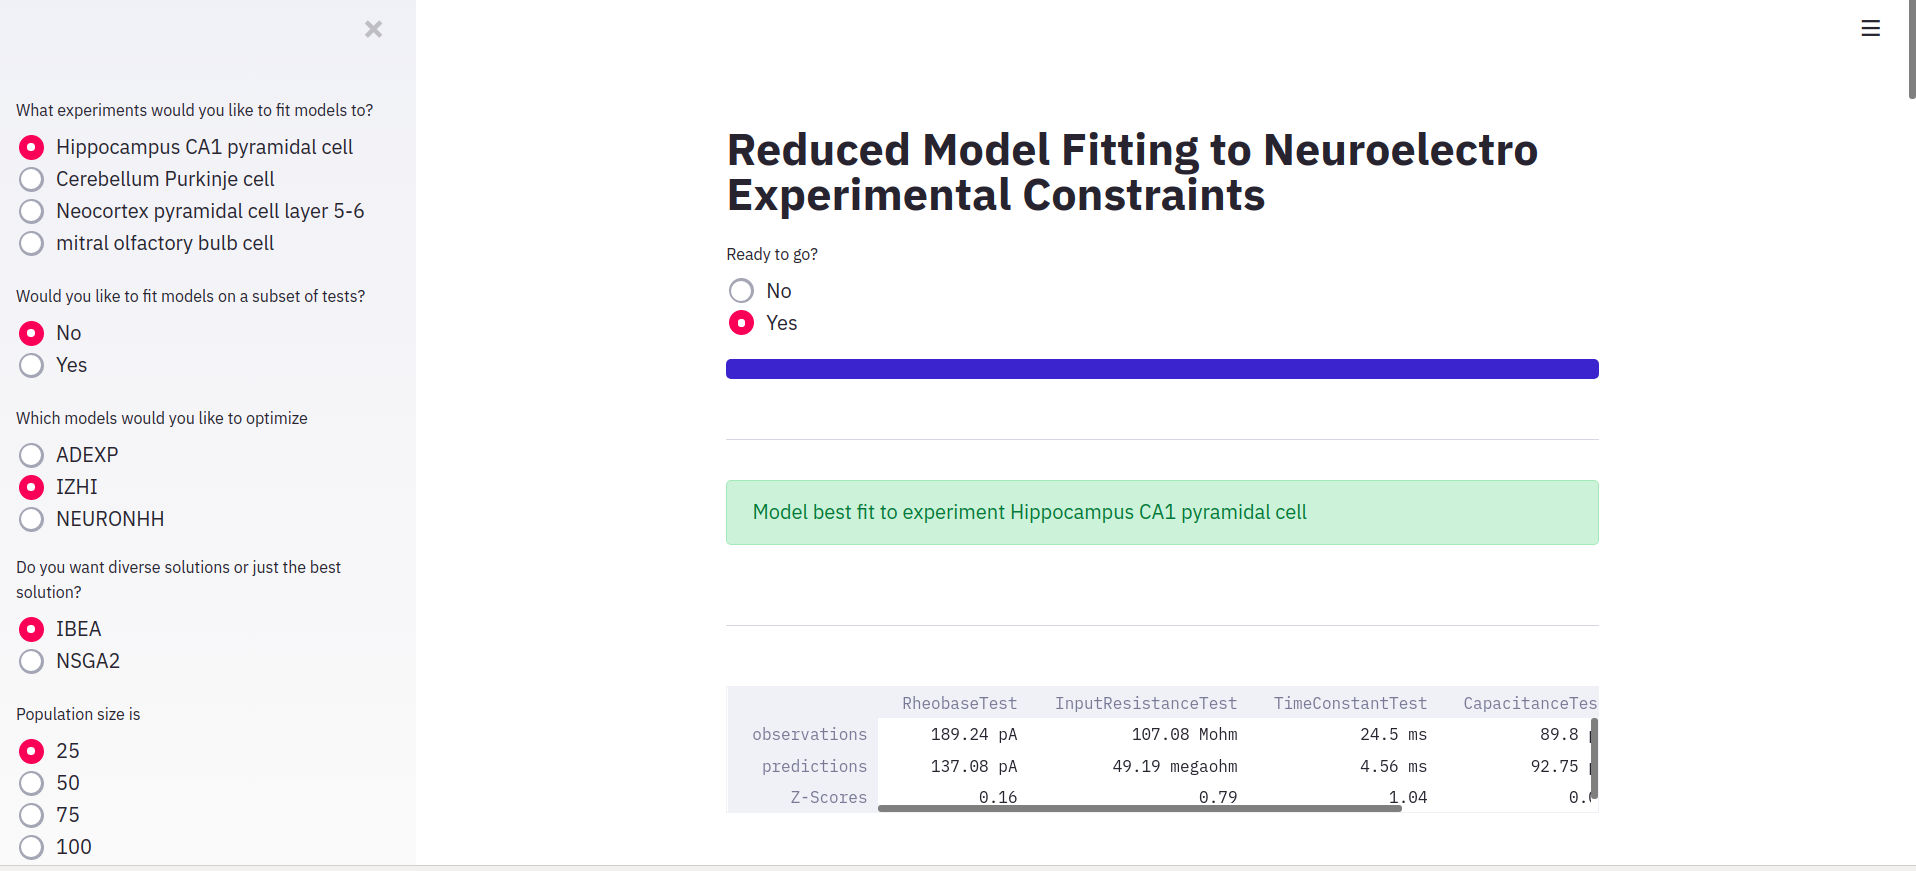
\includegraphics[scale=1]{chapters/app_tex/app_results}
\end{center}
\caption[Web Application (2)]{\textbf{A Web Application for Optimization: Part B}.
Once the optimizer (running on the web server) has completed finished optimizing a model against NeuroElectro data, a table showing model/data agreement is shown to the user.
The user can also optionally scroll through a visualisation of model fitness metrics, such as the $\chi^{2}$ test value.
They can also inspect interactive model waveforms, and download a serialized representation ready to run locally in Python.}
\label{fig:web-app-2}
\end{figure}

When optimization is complete the user is shown the parameters of the optimized model as well as key membrane potential traces (i.e. response to the rheobase current injection) for inspection (Figure \ref{fig:web-app-3}).

\begin{figure}
\begin{center}
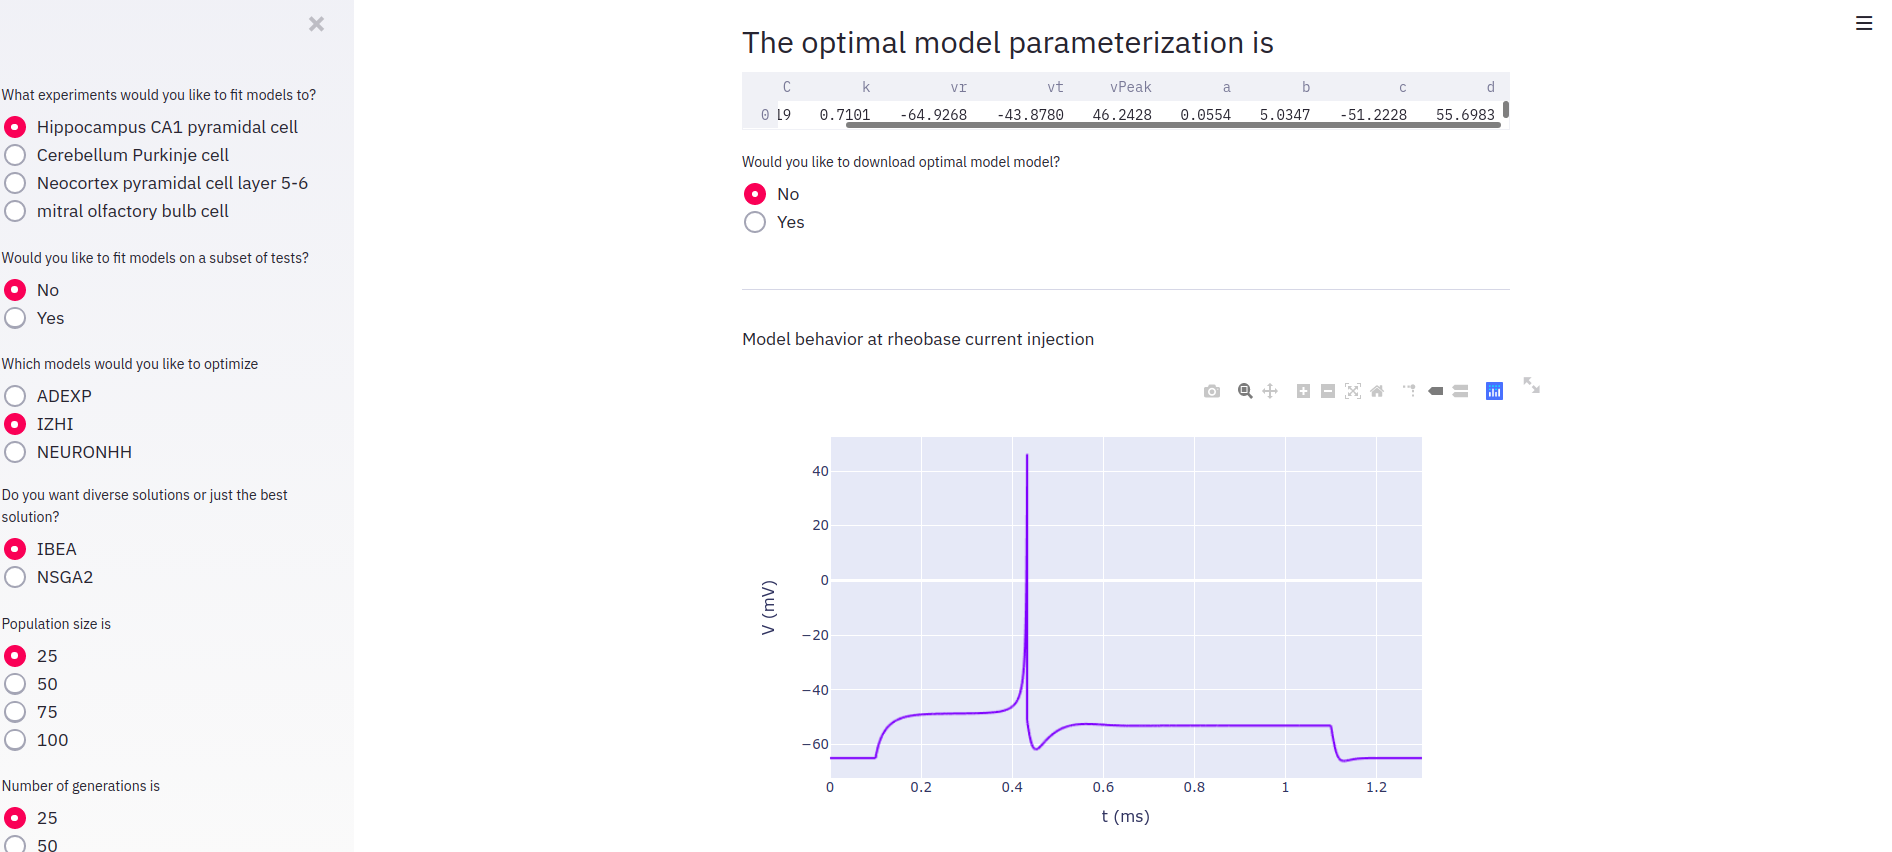
\includegraphics[scale=1]{chapters/app_tex/more_app_results}
\end{center}
\caption[Web Application (3)]{\textbf{A Web Application for Optimization: Part C}.
The application shows an interactive visualisation of the optimized model neuron firing in response to (its computed) rheobase current (shown above), and also under a hyperpolarizing current used to compute other features (not shown above).}
\label{fig:web-app-3}.
\end{figure}

Finally, the user is shown the $\chi^{2}$ statistic (and p-value) for the optimized model, and provided with a link is provided to download these parameters for their own use (Figure \ref{fig:web-app-4}).
Future work will allow the user will be able to download a NeuroML file of the optimized model.

\begin{figure}
\begin{center}
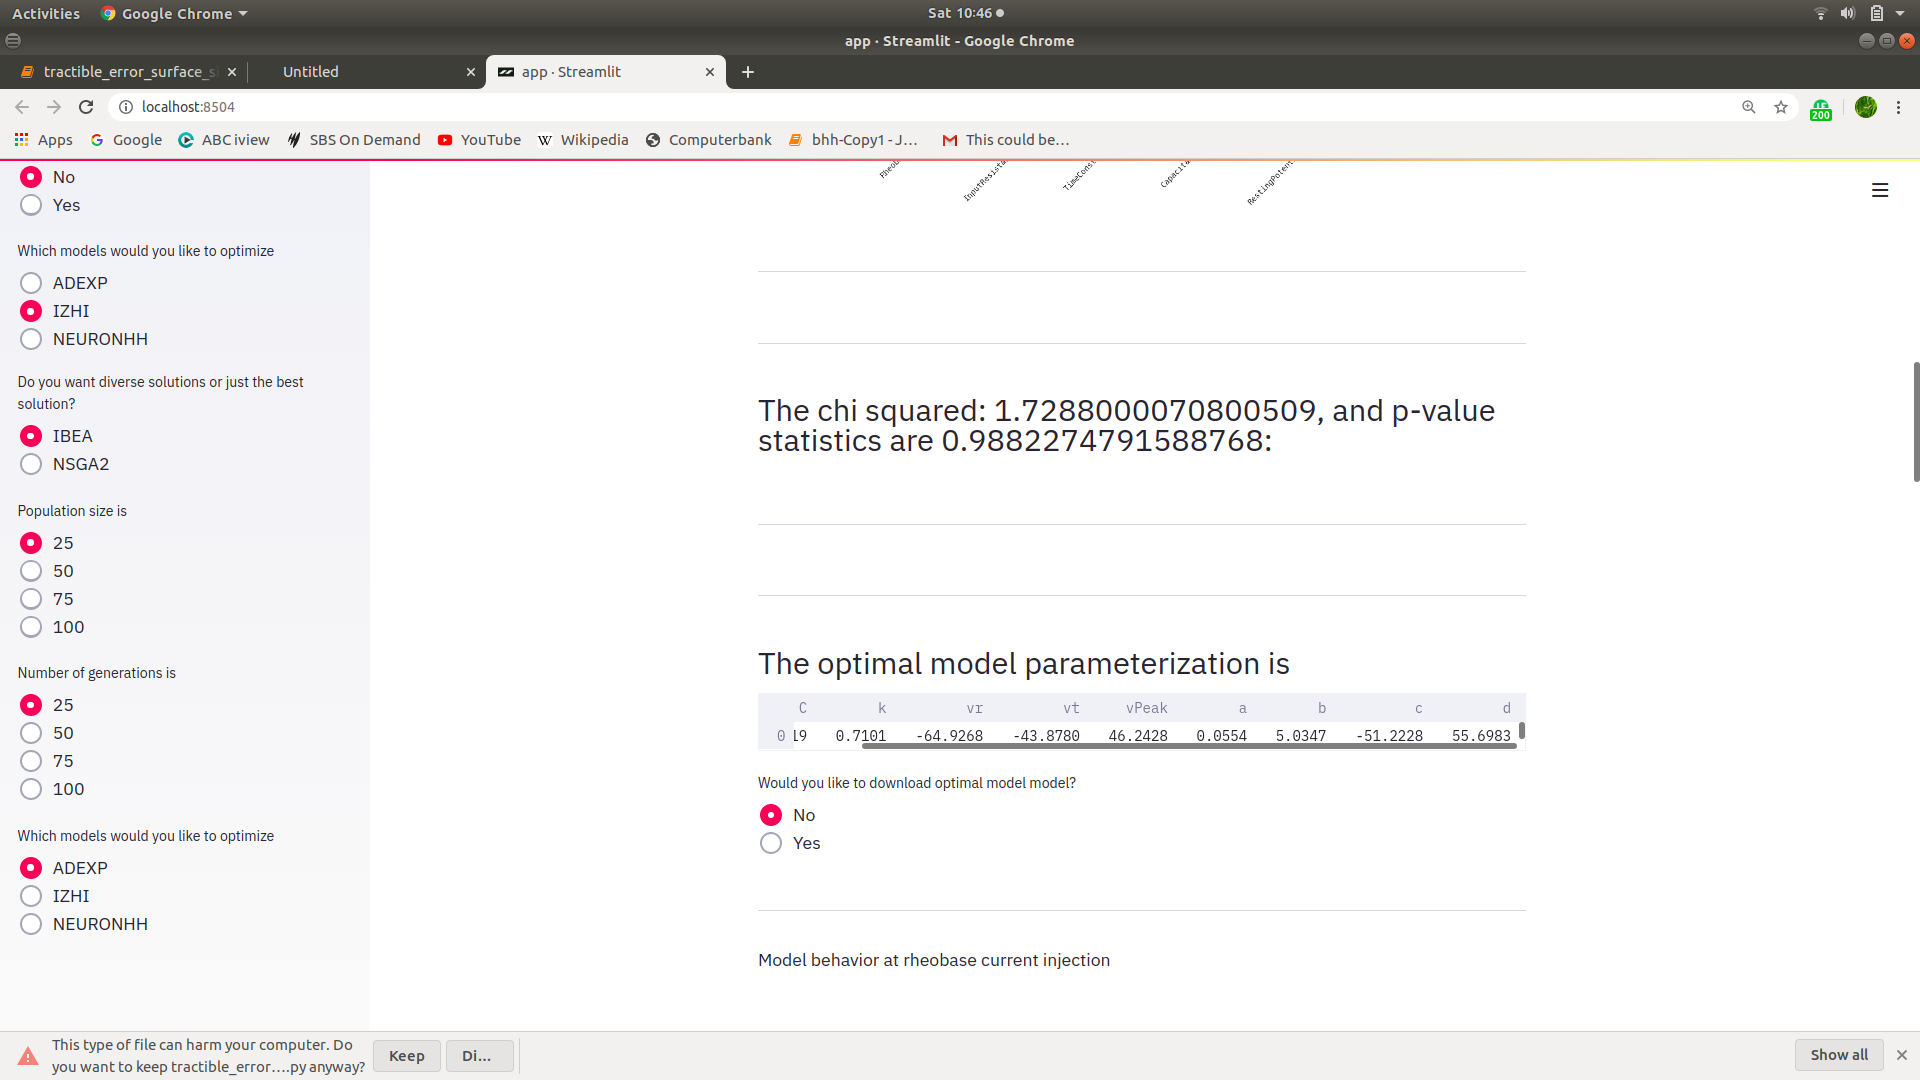
\includegraphics[scale=1]{chapters/app_tex/Screenshot from 2020-09-19 10-46-32}
\end{center}
\caption[Web application (4)]{\textbf{A Web Application for Optimization: Part D}.
The application provides a prompt to download an optimized version of the model. In future work this feature will supportthe download of a NeuroML version of the model for use on alternative simulators.}
\label{fig:web-app-4}.
\end{figure}

Because some of the details of the scoring associated with optimization are unfamiliar to most people, another visualization is provided (Figure \ref{fig:web-app-5} which helps the user visualize the meaning of a Z-score in an optimization context, and displays this information for each feature used to constrain the optimization.
Additional information about the stimuli used and the time taken to run the simulations are also provided.

\begin{figure}
\begin{center}
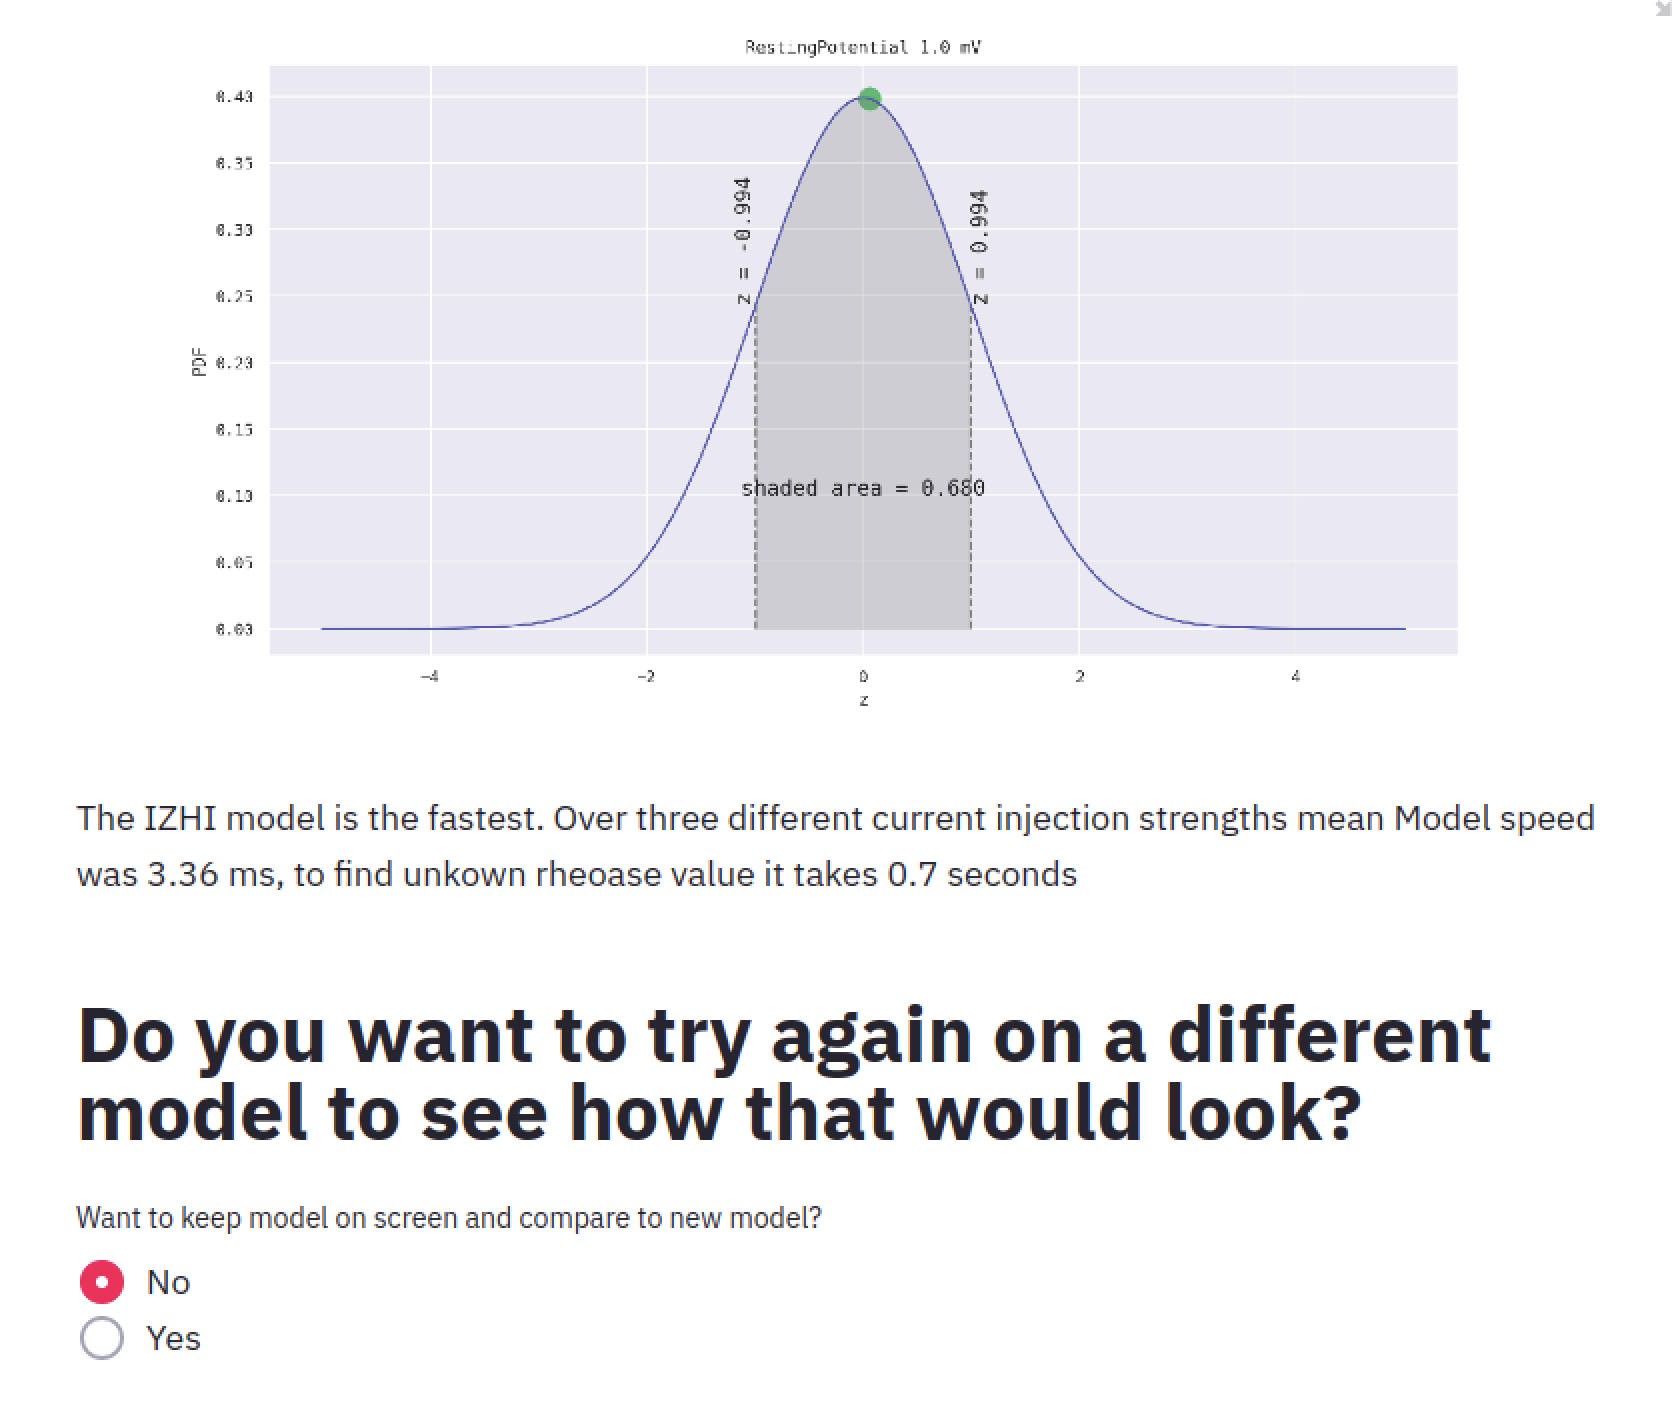
\includegraphics[scale=1]{figures/fixed_white_space.png}
\end{center}
\caption[Web application (5)]{\textbf{A Web Application for Optimization: Part E}.
The application describes additional statistics about the computed features, including an explanation of the Z-score and how it was computed for a given feature.
It also provides information about model performance.}
\label{fig:web-app-5}
\end{figure}
